\documentclass[convert, tikz]{standalone}
%\usepackage{xcolor}
\begin{document}
%\pagecolor[RGB]{255,255,254}
  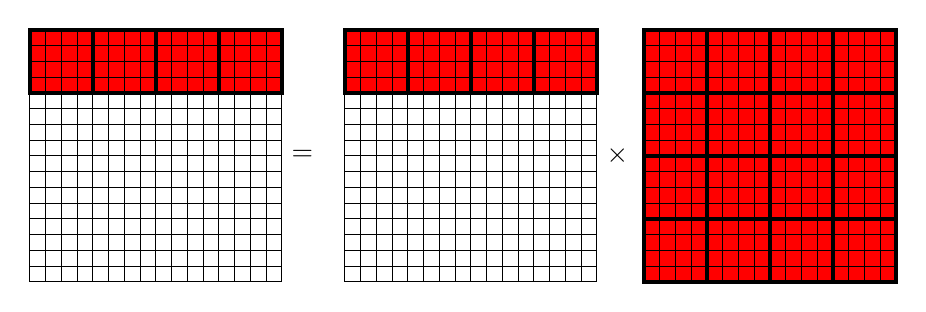
\begin{tikzpicture}[scale=0.2]
    \begin{scope}
      \foreach \i in {0,...,3}{
        \draw[fill=red,ultra thick] (4*\i,12) rectangle (4*\i+4,16);
       }
      \draw[fill=red] (20,15) rectangle (36,16);
      \foreach \i in {0,...,3}{
        \draw[fill=red,ultra thick] (20+4*\i,12) rectangle (20+4*\i+4,16);
       }
      \foreach \i in {0,...,3}{
        \foreach \j in {0,...,3}{
          \draw[fill=red,ultra thick] (39+4*\i,4*\j) rectangle (43+4*\i,4*\j+4);
        }
       }
      \draw(0,0) grid(16,16);
      \draw(20,0) grid(36,16);
      \draw(39,0) grid(55,16);
      \node[right] at (16,8) {$=$};
      \node[right] at (36,8) {$\times$};
    \end{scope}
  \end{tikzpicture}
\end{document}
